\documentclass[12pt,a4paper,oneside]{article}
\usepackage[utf8]{inputenc}
\usepackage[spanish]{babel}
\usepackage[T1]{fontenc}
\usepackage{textcomp}
\usepackage{hyperref}
\usepackage{amsmath}
\usepackage{amsfonts}
\usepackage{amssymb}
\usepackage{graphicx}
\usepackage[utf8]{inputenc}
\usepackage[T1]{fontenc}     % Better font encoding
\usepackage{textcomp}  % For special quotes
\usepackage[left=2.54cm, right=2.54cm, top=2.54cm, bottom=2.54cm]{geometry}
\usepackage{tabularx}
\usepackage{listings}
\usepackage{config/code-style}
\usepackage{config/listing-numbers}
\usepackage{xcolor}
\usepackage{makeidx}
\raggedbottom
\makeindex
\date{\today}

\hypersetup{
	colorlinks=true,
	linkcolor=blue,
	filecolor=magenta,
	urlcolor=cyan,
	pdftitle={Overleaft Example},
}

\usepackage{caption}
\captionsetup[table]{name=Tabla}
\renewcommand*{\lstlistingname}{Exemplo de código}
\renewcommand{\listfigurename}{Figuras}
\renewcommand{\listtablename}{Tablas}

\pagenumbering{arabic}

%Final Python listing configuration
% Biliografia configuracion
\usepackage[
backend=biber,
style=alphabetic,
sortcites,
url=true
]{biblatex}
\addbibresource{bibliography.bib}

\begin{document}
	\begin{titlepage}
	\noindent
	\centering
	\Large {SOFTWARE DEVELOPMENT FULLSTACK}
	\begin{center}
		\centering
		\rule{150 mm}{0.1 mm}
		\Large {BACKEND/FRONTEND\\}
		
		\rule{150 mm}{0.1 mm}
		\large {{Desarrollo Backend/Frontend con Java, JavaScript y PostgreSQL}}
		\rule{150 mm}{0.4 mm}
		\vspace{1 cm}
		\vspace{0.3 cm}
		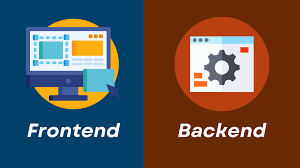
\includegraphics[width=1\textwidth]{image/cover.png}
	\end{center}
	\vspace{0.3 cm}
	\begin{center}
		{\large AUTOR
			{\href{https://github.com/titoroopart/}{@TITOR-OOPART}}}	\\
		{\large YOUTUBE:	{\href{https://www.youtube.com/@ReadToRun}{@ReadToRun}}}	\\
		{\large GITHUB BOOK:  	{\href{https://github.com/titoroopart/Backend_Frontend#}{@Frontend/Backend}}}\\
	\end{center}
	\vspace{0.5 cm}
	\vfill
	\begin{center}
		\large\today
	\end{center}
\end{titlepage}

	\thispagestyle{empty}
	\tableofcontents
	\listoffigures
	\listoftables
	\lstlistoflistings
	\section{[Code01]Instalación de Java JDK y Gradle}
\subsection{Instalación de Java JDK Linux}
\subsubsection{Instalación de Java JDK}
Para instalar java jdk en linux se debe seguir los siguientes pasos:
Instalamos Java JDK
\enablenumbering
\begin{lstlisting}[language=bash]
sudo apt update
sudo apt install default-jdk
\end{lstlisting}
\subsubsection{Configuramos las variables de entorno}
Primero buscamos la ruta exacta de tu JDK

\begin{lstlisting}[language=bash]
ls /usr/lib/jvm/
\end{lstlisting}
Busca el folder exacto de tu JDK (ej: jdk-21-amd64) y agrega la ruta a bashrc con los siguientes comandos.
\begin{lstlisting}[language=bash]
echo 'export JAVA_HOME=/usr/lib/jvm/jdk-21-amd64/' >> ~/.bashrc
echo 'export PATH=$JAVA_HOME/bin:$PATH' >> ~/.bashrc
source ~/.bashrc
\end{lstlisting}
Verificar instalación de Java
\begin{lstlisting}[language=bash]
java -version
javac -version
\end{lstlisting}

\subsubsection{Instalar Gradle}
Con bash
\begin{lstlisting}[language=bash]
curl -s "https://get.sdkman.io" | bash
source "\$HOME/.sdkman/bin/sdkman-init.sh"

sdk install gradle

sdk list

sdk use gradle 8.14
exit
\end{lstlisting}
Correr esto solo si usas fishshell
\begin{lstlisting}[language=bash]
fisher install reitzig/sdkman-for-fish
\end{lstlisting}

Crear una proyecto Gradle
\begin{lstlisting}[language=bash]
mkdir mi-proyecto
cd mi-proyecto
gradle init
\end{lstlisting}
Creamos el proyecto java aplicación y proyecto simple con groovy
Dentro de mi-proyecto deberías ver los siguientes archivos\\
\begin{enumerate}
  \item build.gradle: Archivo de configuración principal de gradle
  \item settings.gradle: Archivo donde se define la configuración del proyecto
  \item src/ Contiene el código fuente y los tests
\end{enumerate}

\subsection{Instalación de Java JDK y Gradle en Windows}
\subsubsection{Descarga e Instala Java JDK}
Descarga Java de su pagina oficial buscando java jdk en google, \url{https://www.oracle.com/java/technologies/downloads/}  para instalar Java JDK Ejecuta el instalador y sigue los pasos (usa la ruta por defecto, ej: 
\begin{lstlisting}[language=bash]
C:\Program Files\Java\jdk-21).
\end{lstlisting}
\subsubsection{Configurar Variables de Entorno} 
\begin{enumerate}
  \item Abre Editar variables de entorno del sistema (busca en el menú Inicio).
  \item En Variables del sistema, haz clic en Nueva y agrega: Nombre: JAVA\_HOME
\\
\begin{lstlisting}[language=bash]
Valor: C:\Program Files\Java\jdk-21 \$(ajusta la version).
\end{lstlisting}
\item Edita la variable Path y agrega:
\begin{lstlisting}[language=bash]
\%JAVA\_HOME\%\bin
\end{lstlisting}
\end{enumerate}
Verificar Java abriendo CMD y ejecuta:
\begin{lstlisting}[language=bash]
java -version
javac -version
\end{lstlisting}
(Debe mostrar la versión instalada).
\\
\subsubsection{Instalar Gradle}
 Descarga Gradle desde \url{https://gradle.org/install/#manually} (versión "Binary-only"). Extrae el ZIP en la siguiente ruta crear carpeta Gradle en el disco C:
\begin{lstlisting}[language=bash]
 C:\Gradle\gradle-8.14
\end{lstlisting}
Configurar Variables de Entorno para Gradle\\
En "Variables del sistema", Edita Path y agrega:
\begin{lstlisting}[language=bash]
C:\Gradle\gradle-8.14\bin
\end{lstlisting}
	\section{[Code02] APIconsumer con java + gradle + Retrofit}

Una API (Aplication Programming Interface) es un una interfase que permitirá a los programas comunicarse compartiendo las funcionalidades, datos, etc. Esto facilita a los desarrolladores a disponer de muchas herramientas y base de datos disponibles y usarlos en sus aplicaciones ya sea conectándose a sus propios servidores o a servidores de terceros.
\\
Un ApiConsumer sera esa parte del código que nos permitirá conectarnos a una API del lado del servidor.\\
Para crear un API consumer necesitaremos lo siguiente:
\begin{enumerate}
  \item Elegir un lenguaje de programación en este caso Java21
  \item Una librería, En el caso de Java retrofit
  \item Configurar los http methods get, post, put, delete
  \item Agregar content type Authorization
  \item Definir el body en el caso de los métodos post put y delete
  \item Manejar la respuesta o el error de la petición
\end{enumerate}
En el caso de Java21 trabajaremos con la librería retrofit, para agregar esta libreria a un poryecto gradle groovy simplemente agregamos la dependencia a build.gradle

\begin{lstlisting}[language=java]
dependencies {
  \\ otras dependencias
    implementation 'com.squareup.retrofit2:retrofit:2.9.0'
    implementation 'com.squareup.retrofit2:converter-scalars:2.9.0'
}
\end{lstlisting}
Construimos un objeto retrofit basado en la siguiente documentación \url{https://square.github.io/retrofit/2.x/retrofit/}
\begin{lstlisting}[language=java]
// archivo app/src/main/java/ApiConnection.java
import retrofit2.Retrofit;
import retrofit2.converter.scalars.ScalarsConverterFactory;

public class ApiConnection {

  public static void connection(){
    Retrofit retrofit = new Retrofit.Builder()
      .baseUrl("https://api.example.com/")
      .addConverterFactory(ScalarsConverterFactory.create())
      .build();
  }
}
\end{lstlisting}
Con import importamos todas las librerías necesarias, luego con .Builder() a la hora de crear el objeto iniciamos el patrón de diseño builder para construir el objeto retrofit, los .baseUrl() y .addConverterFactory() son parámetros necesarios para construir el objeto y por ultimo .build() es la orden que construye el objeto retrofit.
\\
El metodo .addConverterFactory es importante para poder manejar el objeto serializado y desealizarlo en un string json etc.
\\
Para poder generar el request es necesario usar una interface para el endpoint, esta interfase sera capas de manejar las peticiones get, post, put, delete etc y recibir variables si así lo requiere ej endpoint random:
\begin{lstlisting}[language=java]
import retrofit2.http.GET;
import retrofit2.Call;

  public interface getConnection {
    @GET("random")
    Call<String> getPost();
}
\end{lstlisting}
Ejemplo interface con parámetro id en el endpoint.
\begin{lstlisting}[language=java]
import retrofit2.http.GET;
import retrofit2.http.Path;
import retrofit2.Call;

  private interface GetList {
      @GET("posts/{id}")
      Call<String> getPost(@Path("id") int id); // Retorna String en lugar de objeto
  }
\end{lstlisting}


	\printbibliography[heading=bibintoc]
\end{document}
